\documentclass{article}
\usepackage[utf8]{inputenc}

%\title{Joystick-controlled-laser}
%\author{mo000007 }
\usepackage[left=3cm, right=3cm, top=3cm]{geometry}
\usepackage{graphicx}
\begin{document}

%\maketitle

\begin{center}
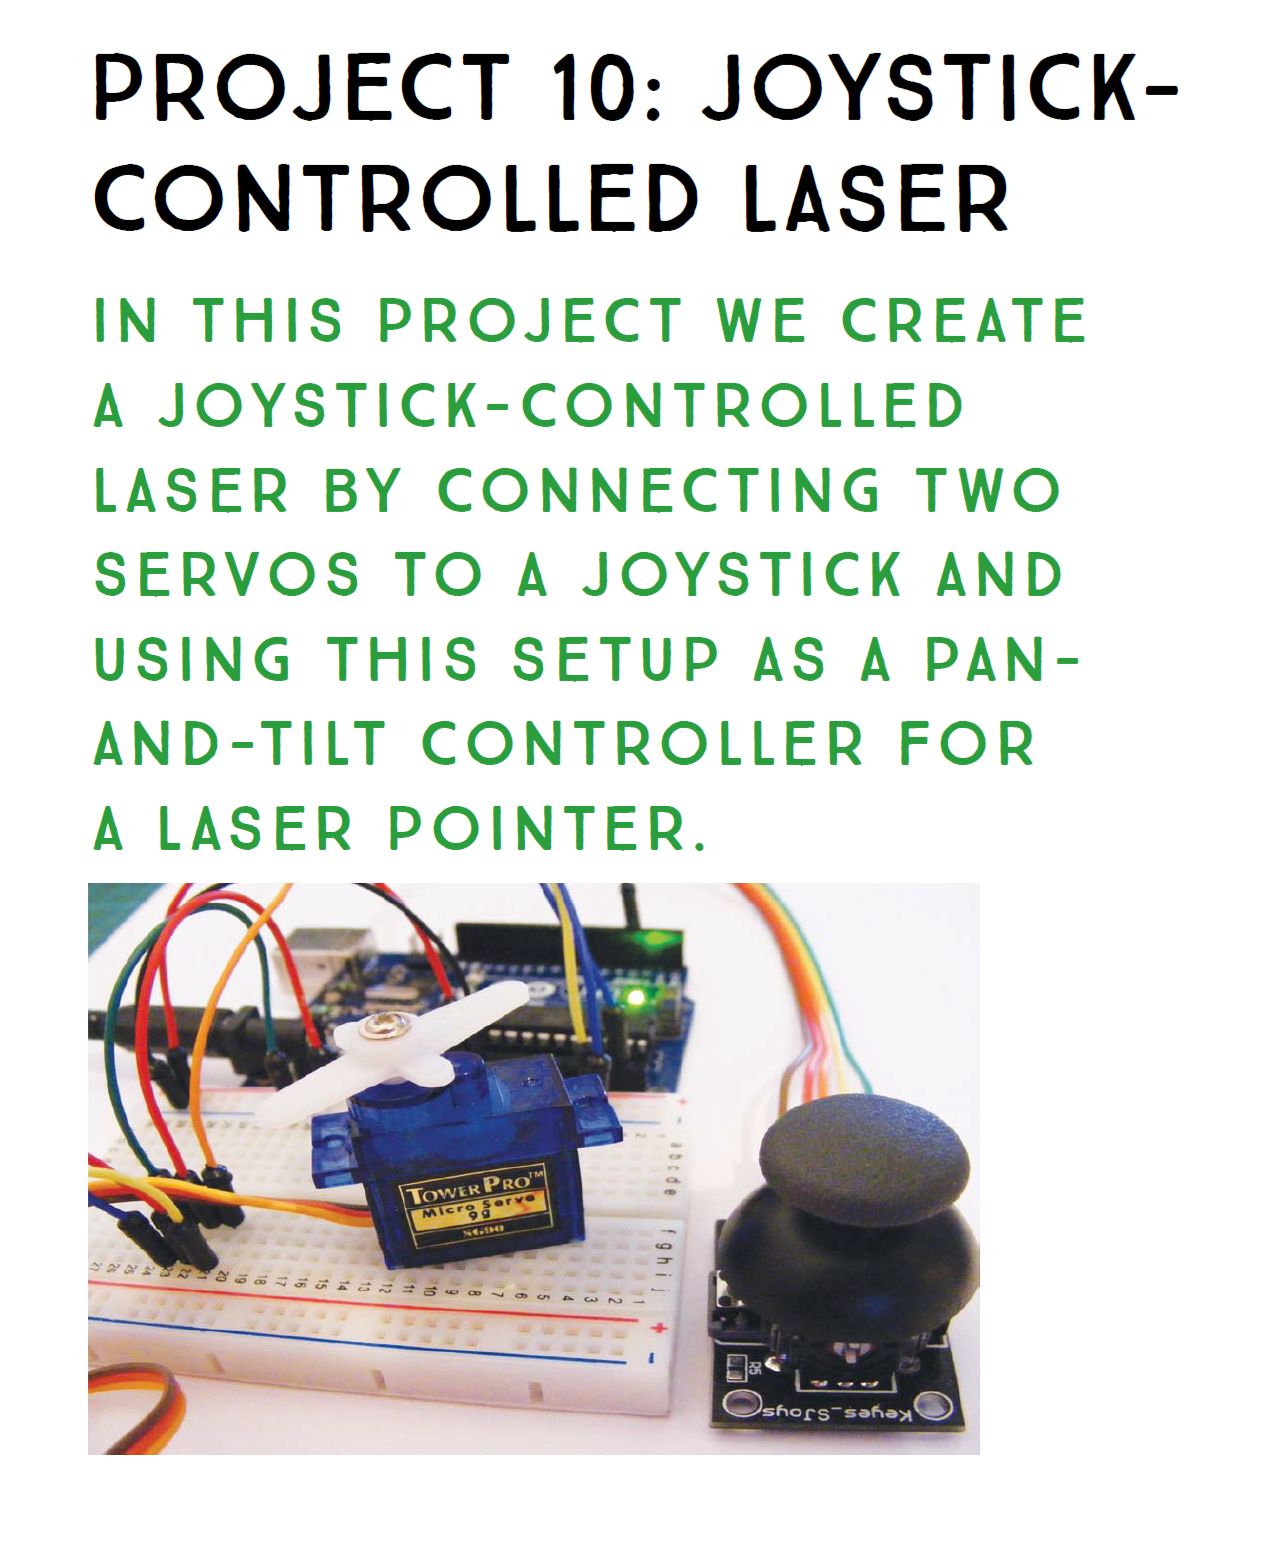
\includegraphics[width=\textwidth, height=20cm]{title.png}
\end{center}

\begin{center}
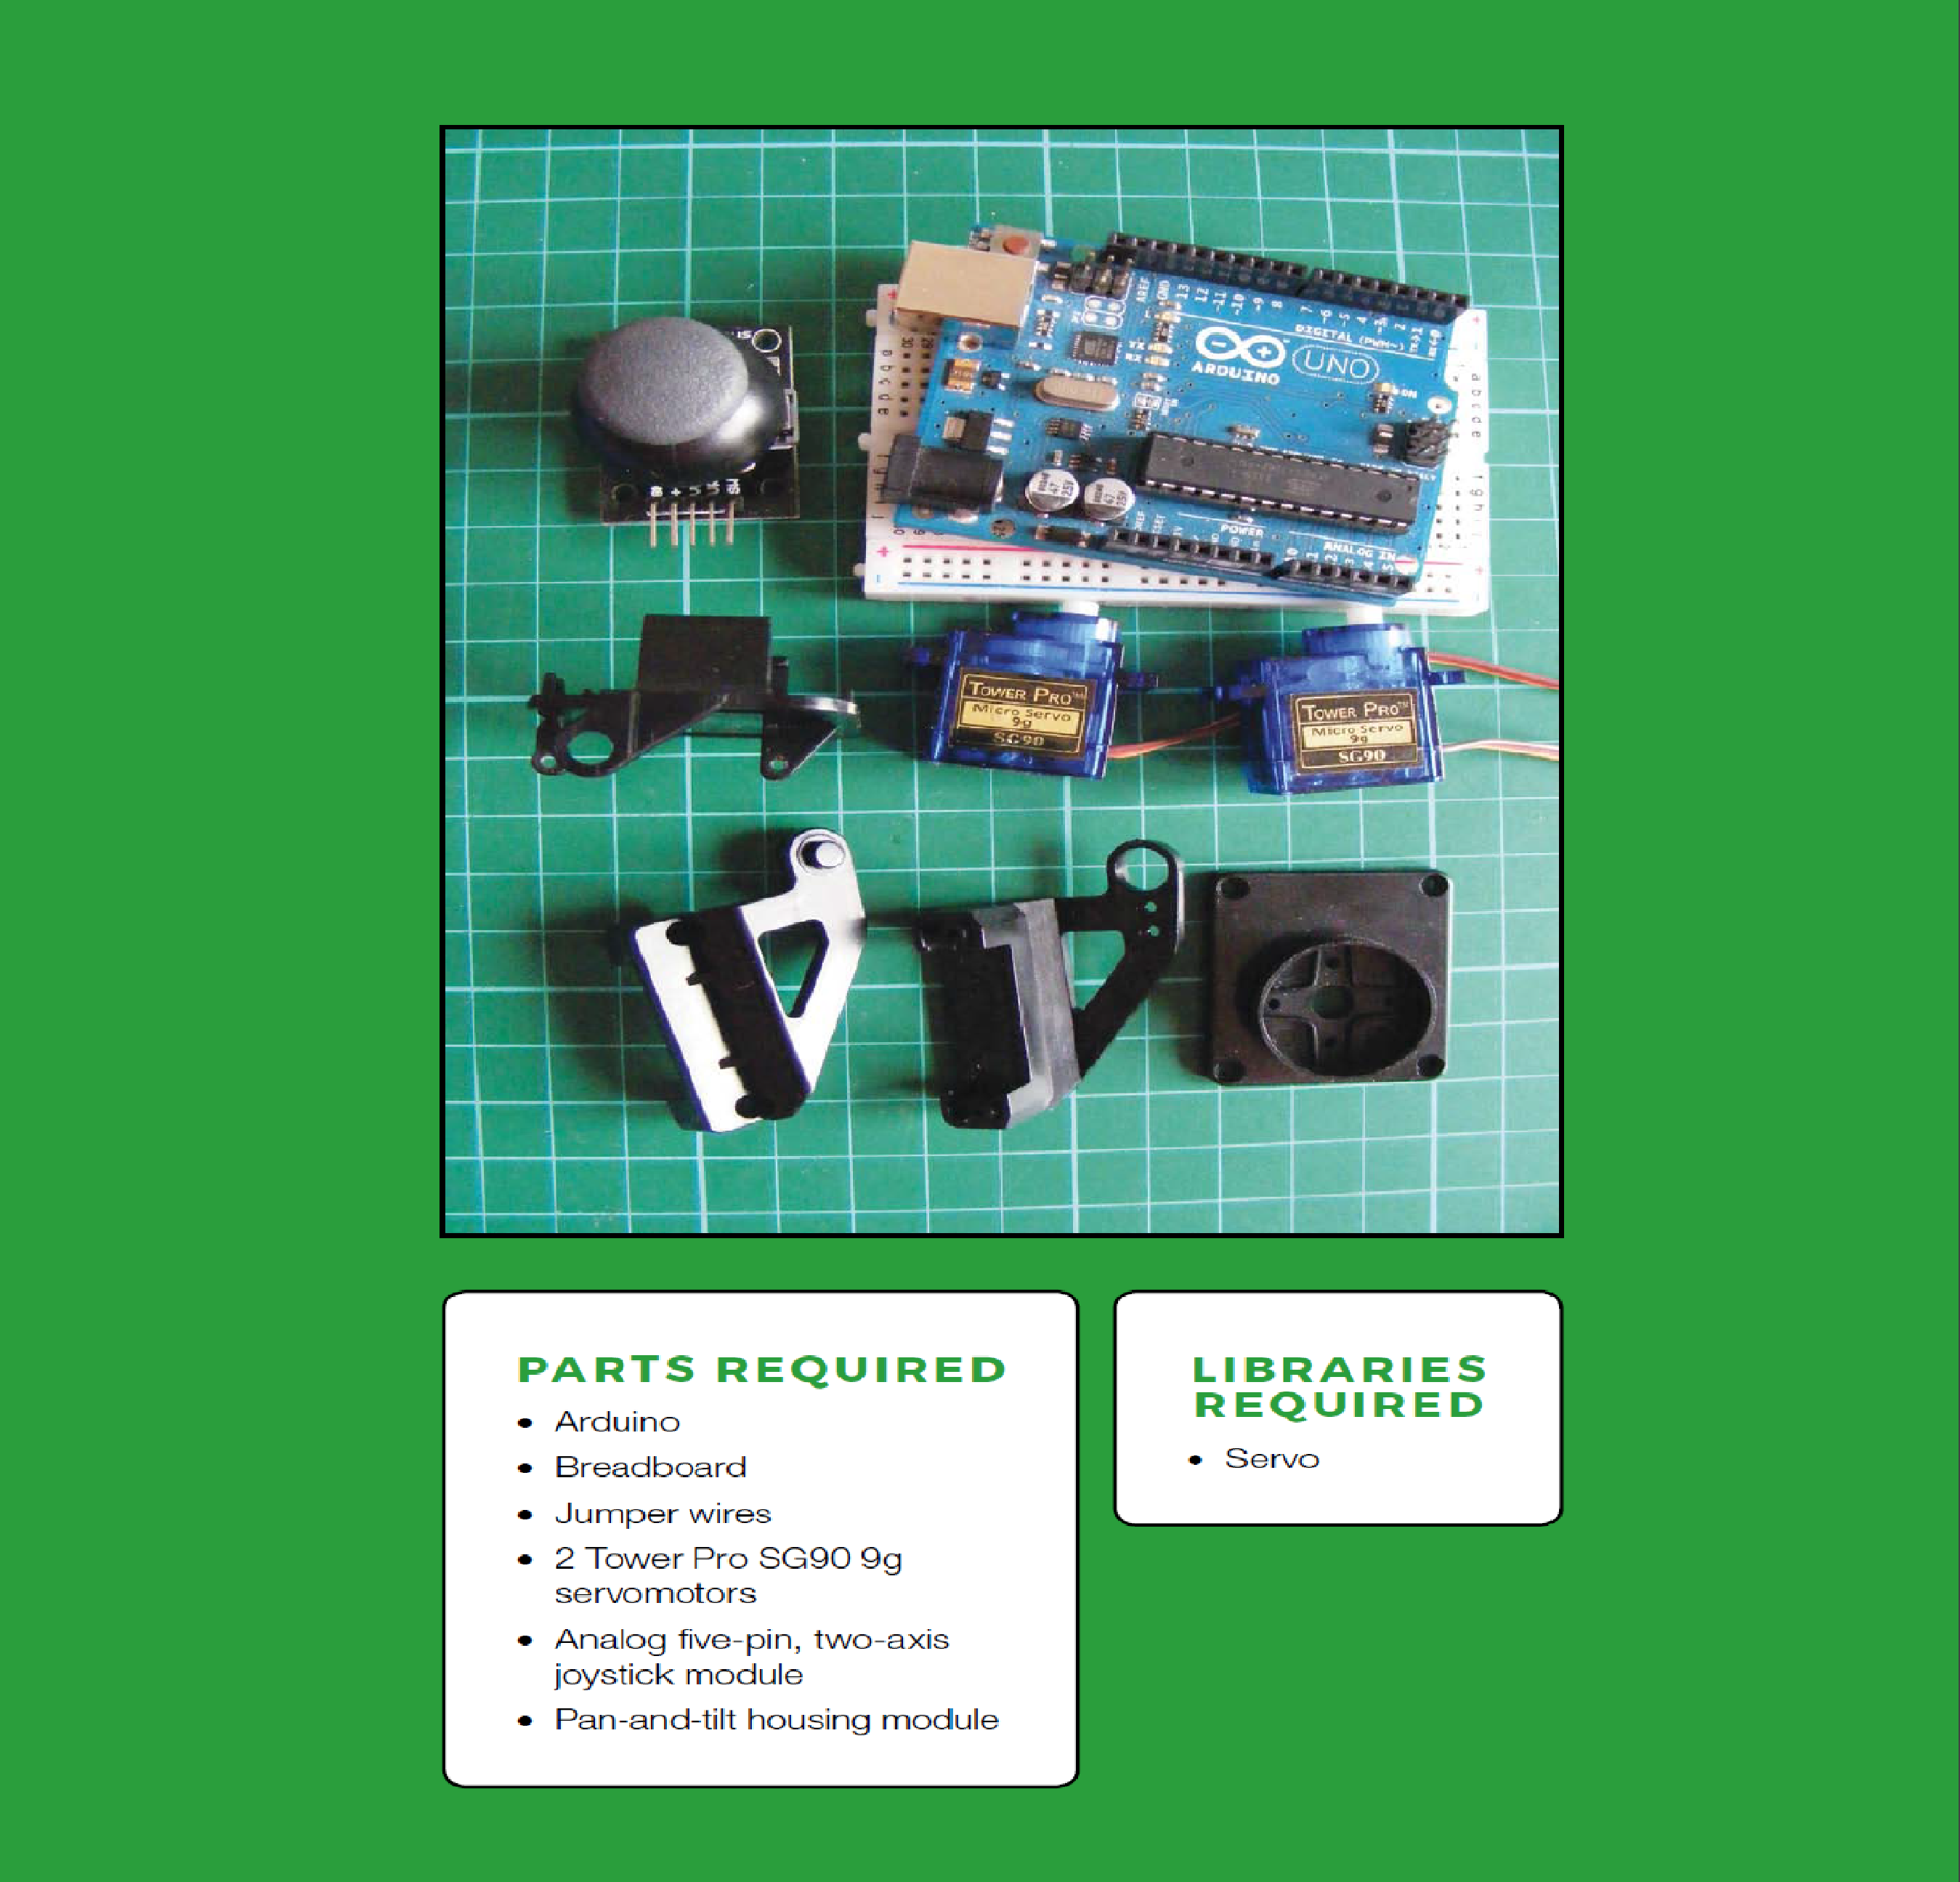
\includegraphics[width=\textwidth, height=18cm]{requir.png}
\end{center}

\section{Setup}
First you will need to download, unzip, and install the Arduino Integrated Development Environment
(IDE) from https://www.arduino.cc/en/Main/Donate (does not need admin privileges).

\section{Objectives}
By the end of this session, students should be able to:

\begin{itemize}
\item Describe the mechanical, electrical, and programming parts of joysticks and servos at a high
  level to someone unfamiliar with them.
\item Understand how pushbuttons work and why it is necessary to debounce them in many cases.
\end{itemize}

\section{How it Works}
Servos are small motors that can precisely angle their arms to positions between 0 and 180
degrees. In this project we will place the servos into a tilt-and-pan mount. The tilt-and-pan mount
makes it much easier to attach the laser to the servo. For this project we are controlling a laser,
but you could easily replace the laser with a web-cam or other small devices. We will be using two
servos: one for left and right movement, and the other for up and down movement.

The joystick is basically two potentiometers and a button that allows us to measure the movement of
the stick. The potentiometers are variable resistors that know their value, which for this
experiment is between 0 and 1,023. As you move the joystick around its center, the potentiometers
decide how far the servos move depending on the rotation of the joystick.

When the joystick is moved to the left or right, the corresponding servo will move in that
direction; when the joystick is moved up or down, the other servo will move up or down.

\section{Building the Circuits}
The schematic for the circuits you will be building is below. First, we will connect the servos and
the joystick to the Arduino.

\begin{center}
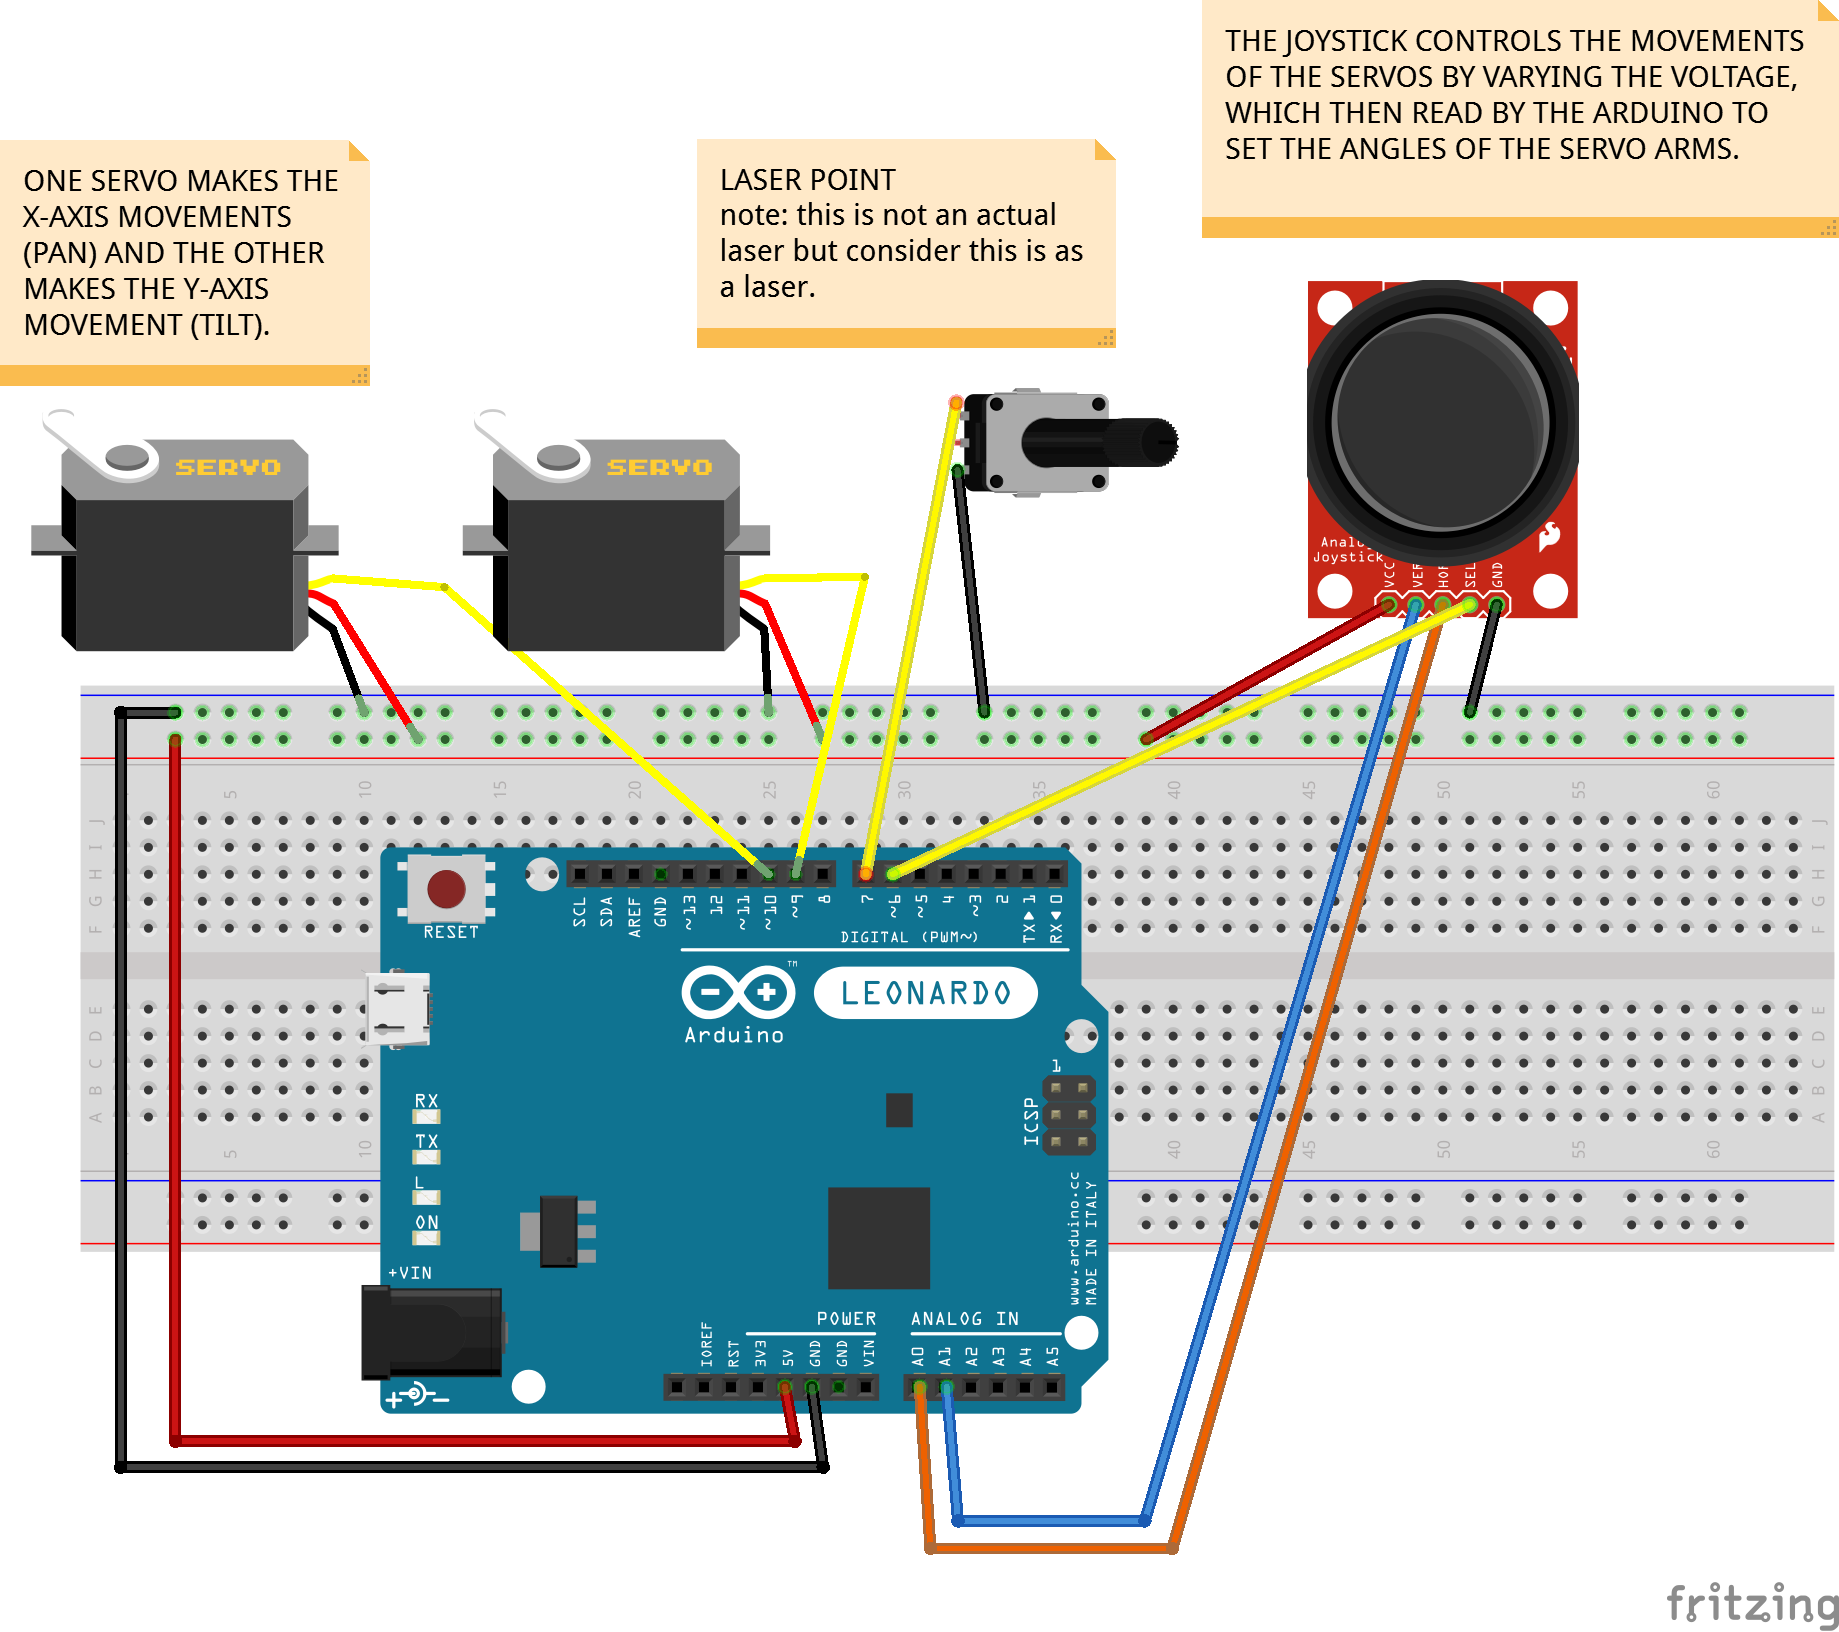
\includegraphics[width=\textwidth]{diagram.png}
\end{center}

Then, we will attach the laser diode to the top of the module either using a glue gun for a
permanent fixture, or using tape if you want something more temporary. Take the X position servo and
make it the base of the turret. Then lay the Y position servo on its side on top of the X position
servo and tape it to the servo arm. Next mount the laser on the Y position servo so that it’s arm
would move up and down with the laser. Now you can control the laser using the joystick. The servos
will clip into the tilt-and-pan module as shown in the figure below. Note that the \emph{brown} wire
on the servo is ground, the \emph{red} one is power, and the \emph{yellow-orange} one is the input
signal to the servo.

\begin{center}
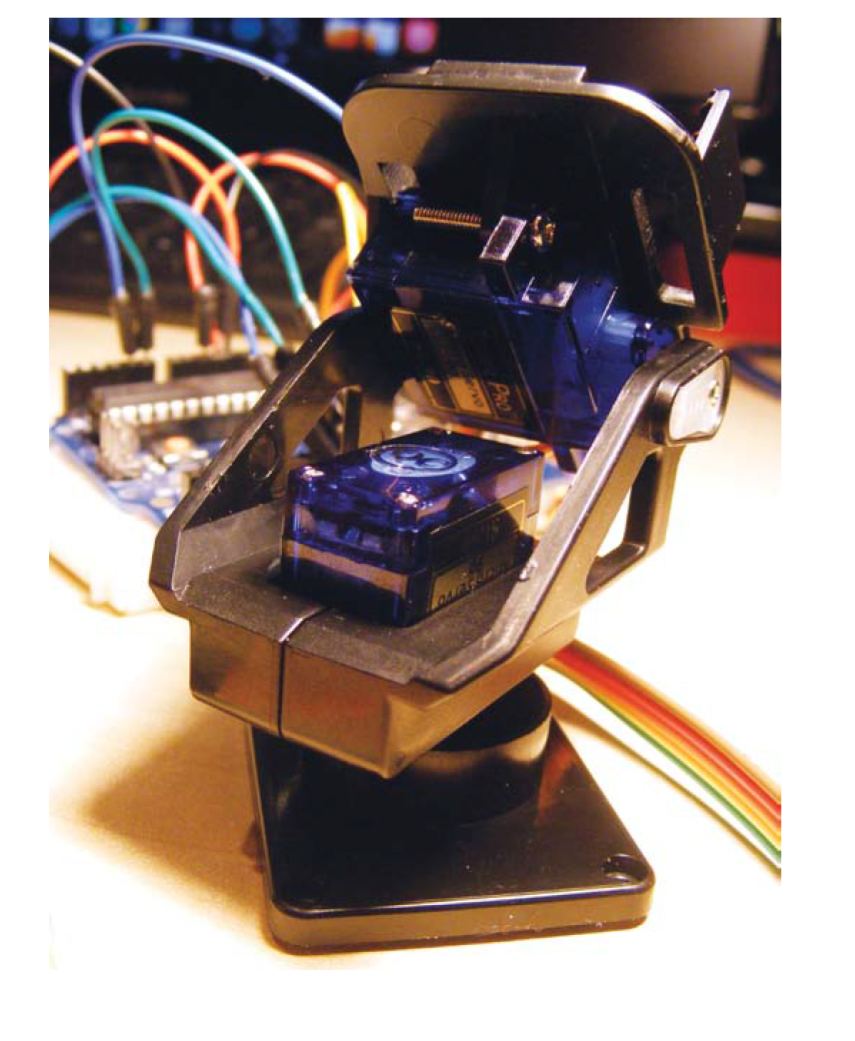
\includegraphics[width=6cm]{laser.png}
\end{center}

\section{Programming the Arduino}
The base code for programming the Arduino is provided. Using the Arduino IDE, open the .ino file.
The IDE allows you to do 4 things: edit the code, verify the code (i.e. does not contain syntax
errors), upload the code to the Arduino, and view the diagnostic output of things as they run on the
Arduino.  Uploading to the Arduino is easy! Just click the Upload arrow in the IDE.

\section{Tuning the Code}
First we call on the Servo library and then defines the two servos as tilt and pan. The joystick
x-axis is attached to Arduino pin A0 and the y-axis to Arduino A1, and these are our INPUT. The x-
and y-axes are then set as variables for movement. The tilt servo is attached to Arduino pin 9 and
pan is attached to Arduino pin 10, and these are our OUTPUT. The Arduino then reads the INPUT from
the joystick and changes this voltage to OUTPUT, moving the servos according to which direction is
chosen.

\section{ Extending the Code}
Once you have the joystick-controlled laser working, let’s try to press the button on the joystick
to turn on or turn off the laser. What happens when you try that? Kind of jerky/inconsistent right?
We need to ``debounce'' the button we press, so that the Arduino more reliably reads the correct
state of the button from the joystick. Debouncing is the process of (1) checking the state of a
button at a given time, (2) checking it again later and see if it has the same state, (3) treating
the read value as the correct state of the button if and only if (1) and (2) are true.

There is already a function in the code that can perform debouncing, all you need to do is to modify
the code slightly to use it!

\end{document}
